\documentclass{report}
\usepackage{amsmath}
\usepackage{graphicx}
\usepackage{subcaption}
\usepackage{float}
\usepackage{caption}
\usepackage[top=0.8in,bottom=0.8in,left=0.8in,right=0.8in]{geometry}
\usepackage[framed,numbered,autolinebreaks,useliterate]{/Applications/TeX/mcode}
\usepackage{fancyhdr}


\title{ME354: Experimental Methods in Fluids Mechanics \\[10pt] \large Final Project: Bringing Life To Images \\ \large{Autumn 2013}}
\author{David Manosalvas \\[2pt] Mehul Oswal}
\date{}
\begin{document}
\maketitle
\pagestyle{fancy}
\lhead{Autumn'13}
\chead{ME354 Project Report}
\rhead{Manosalvas \& Oswal}
\tableofcontents
\chapter{Introduction}
Removing noise from an original signal is a challenging problem receiving due attention from researchers. Digital images play an important role in experimental research and images acquired are often blurry and noisy. Thus prior to analyzing image data, denoising and sharpening becomes necessary. This project aims to explore some of the widely used image enhancement algorithms to sharpen images and implement a robust metric to quantify the performance of filters under different blur sources.\\

\noindent {\bf Mathematical theory behind image processing: }\\
Blurred images are modeled as the true image convolved with a point spread function plus additive noise. The point spread function (PSF) that convolves the true image is generally a property associated with the optics that have contributed to the blur while noise can be due to poor illuminance, quantization among other sources. Mathematically, a blurry image can be represented as follows\\
\begin{equation}
v(m,n)= h(m,n) \star u(m,n) + \eta(m,n)
\end{equation}
where, $u(m,n)$ is the true image, $h(m,n)$ is the PSF, $\eta(m,n)$ is the additive noise and $v(m,n)$ is the blurry image. Image sharpening involves calculating an estimate of the true image $\hat{u}(m,n)$ using filters.
\begin{equation}
\hat{u}(m,n)= g(m,n) \star v(m,n)
\end{equation}
Filters calculate function $g(m,n)$ using some knowledge of the PSF causing the blur and an estimate of the signal to noise ratio.\\

\noindent {\bf Experimental \& Analysis set up: }\\
The experimental and analysis setup for this project is as depicted in the following figure.
\begin{figure}[h!]
  \centering
                \centering
                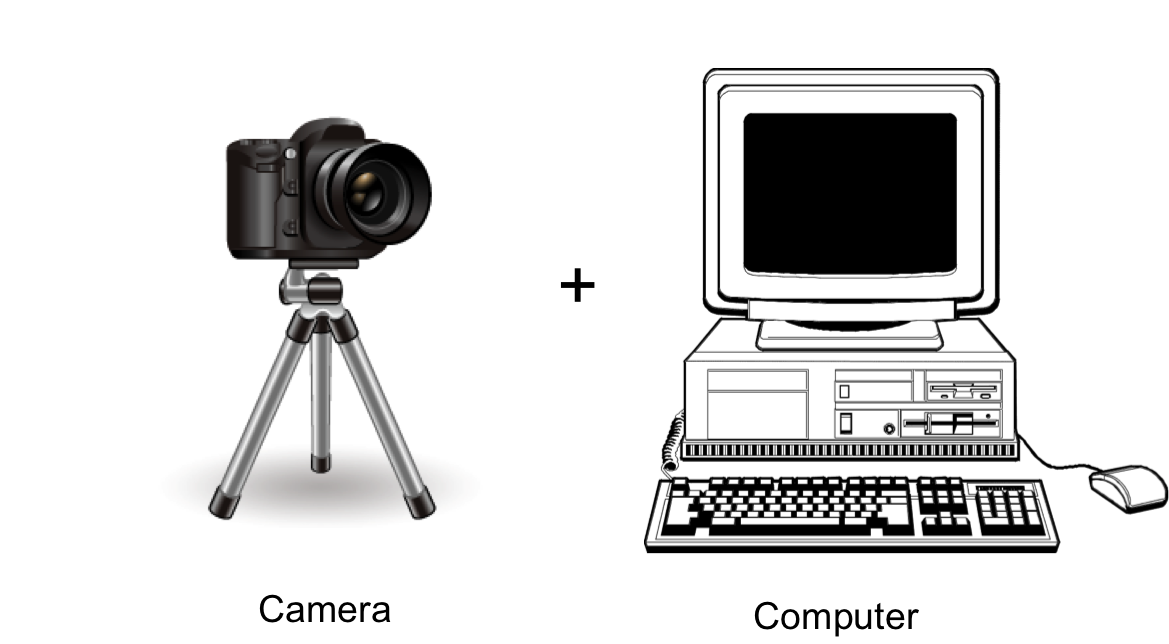
\includegraphics[width=.5\textwidth]{experimental_setup.png}
                \caption{Experimental setup consists of a good camera and a computer system. The camera captures images under pre-defined settings like focal length, shutter speed, aperture size and luminance while computer has been used to perform image enhancement \& filter analysis.}
                \end{figure}

\chapter{Filter Characteristics}
 Choice of filter is very important in image restoration and restored image characteristics. This part of the project aims to study different filters and compare their enhancement effectiveness and deblur characteristics under various simulated and real image blur phenomenon. Before we present a comparison, let us briefly discuss the different filters studied for the purposes of this project. Various filters compared are, 
\begin{enumerate}
\item Inverse and Pseudo filter
\item Wiener filter
\item Geometric mean filter
\item Constrained least squares filter
\end{enumerate} 
Mathematical formulation of these filters has been presented in the Appendix and will not be discussed here. 
\section{Train Image: Supersonic flow around a sphere}
In this simulated motion blur, train image was procured from Van Dyke's Album of Fluid Motion and depicts the formation of shock around a sphere at flow Mach no. 3. This image was blurred using a motion PSF and had Gaussian white additive noise. The blurred image and recovered image are presented below. Filter deblur characteristics follow below.

\begin{figure}
        \centering
        \begin{subfigure}[b]{0.4\textwidth}
                \centering
                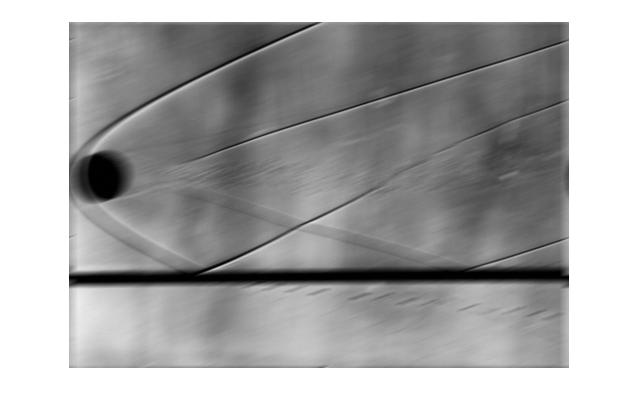
\includegraphics[width=\textwidth]{/Users/mehuloswal/me354_final_project/report/part1_figs/ssphere_motion.jpg}
                \caption{Blurry image}
                
        \end{subfigure}
        \begin{subfigure}[b]{0.4\textwidth}
                \centering
                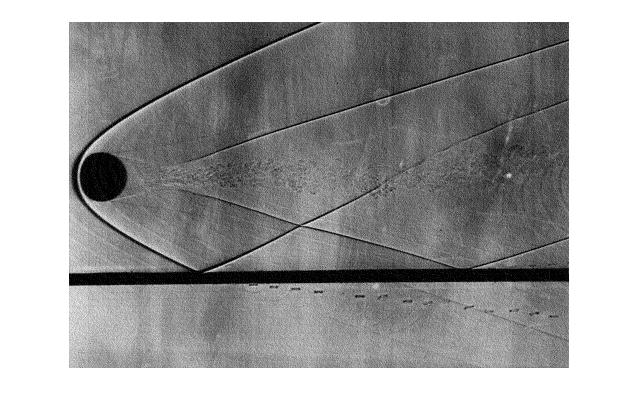
\includegraphics[width=\textwidth]{/Users/mehuloswal/me354_final_project/report/part1_figs/ssphere_wiener.jpg}
                \caption{Wiener filter sharpened image} 
        \end{subfigure}
\caption{Image enhancement on the blurred image was performed using all the filters. For representative purposes only the sharpened image using Wiener filter has been shown here. Blur PSF used for this simulation represented blur effect due to motion. Variance of the additive noise is of $O(10^{-5}$. }
\end{figure}

\begin{figure}[h!]
  \centering
                \centering
                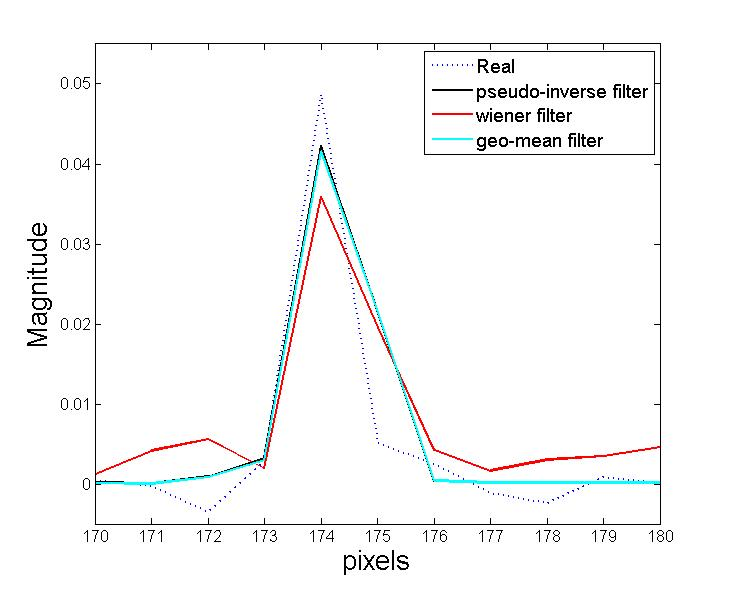
\includegraphics[width=.5\textwidth]{/Users/mehuloswal/me354_final_project/report/part1_figs/kernel_motion.jpg}
                \caption{Kernel comparison for blur due to motion}
                \end{figure}

\begin{figure}
        \centering
        \begin{subfigure}[b]{0.4\textwidth}
                \centering
                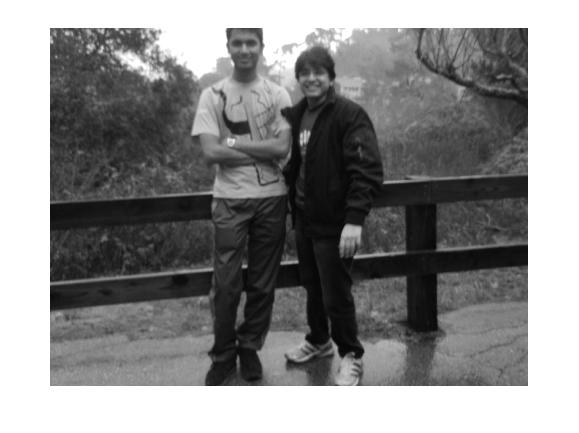
\includegraphics[width=\textwidth]{/Users/mehuloswal/me354_final_project/report/part1_figs/blur_personal.jpg}
                \caption{No reference blurry image}
                
        \end{subfigure}
        \begin{subfigure}[b]{0.4\textwidth}
                \centering
                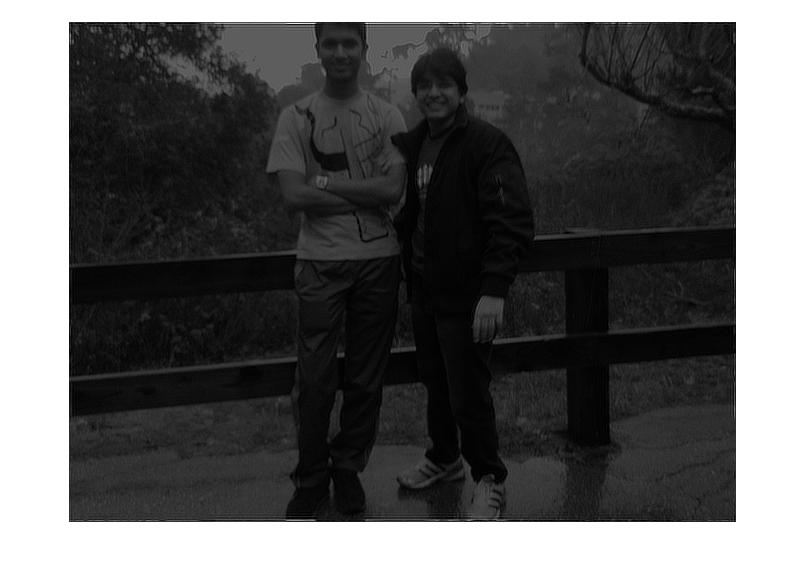
\includegraphics[width=\textwidth]{/Users/mehuloswal/me354_final_project/report/part1_figs/sharp_personal.jpg}
                \caption{Wiener filter sharpened image} 
        \end{subfigure}
\caption{No reference image enhancement}
\end{figure}


\chapter{Sharpness metric}
\chapter{Project Summary}


%\begin{figure}
%        \centering
%        \begin{subfigure}[b]{0.4\textwidth}
%                \centering
%                \includegraphics[width=\textwidth]{Mach_number_2}
%                \caption{Mach number surface plot}
%                
%        \end{subfigure}
%        \begin{subfigure}[b]{0.4\textwidth}
%                \centering
%                \includegraphics[width=\textwidth]{c-mach}
%                \caption{Mach number contour plot} 
%        \end{subfigure}
%\caption{Mach Number}
%\end{figure}

\newpage
\chapter{Appendix}
\section{Additional Results}
\section{Matlab Codes}
\subsection{Master script}
%\lstinputlisting{Driver_prob1.m}
\section{References}
\begin{enumerate}
\item 
\item
\end{enumerate}
\end{document}